\documentclass[11pt]{article}

% Packages for better typography and formatting
\usepackage[utf8]{inputenc}  % Handle UTF-8 encoding
\usepackage[T1]{fontenc}     % Better font encoding
\usepackage{lmodern}         % Improved font
\usepackage{microtype}       % Better spacing
\usepackage{geometry}        % Adjust margins
\usepackage{amsmath, amssymb} % Math symbols and formatting
\usepackage{graphicx}        % Include graphics
\usepackage{hyperref}        % Hyperlinks
\usepackage{enumitem}        % Customizable lists
\usepackage{xcolor}          % Color text
\usepackage{tcolorbox}       % Colored boxes
\usepackage{tikz}
\usepackage{caption}
\usepackage{multicol}
\usepackage{titlesec}
\usepackage[parfill]{parskip} % Use parskip package without extra space
\titlespacing*{\subsection}{0pt}{\subsecbeforeskip}{\subsecafterskip}

% Geometry settings for better note-taking space
\geometry{
  a4paper,
  left=0.5in,
  right=0.5in,
  top=0.5in,
  bottom=0.5in,
}

% Define the lengths for before and after spacing
\newlength{\subsecbeforeskip}
\setlength{\subsecbeforeskip}{8ex}
\newlength{\subsecafterskip}
\setlength{\subsecafterskip}{1.5ex}


%From M275 "Topology" at SJSU
\newcommand{\id}{\mathrm{id}}
\newcommand{\taking}[1]{\xrightarrow{#1}}
\newcommand{\inv}{^{-1}}

%From M170 "Introduction to Graph Theory" at SJSU
\DeclareMathOperator{\diam}{diam}
\DeclareMathOperator{\ord}{ord}
\newcommand{\defeq}{\overset{\mathrm{def}}{=}}

%From the USAMO .tex files
\newcommand{\ts}{\textsuperscript}
\newcommand{\dg}{^\circ}
\newcommand{\ii}{\item}

% % From Math 55 and Math 145 at Harvard
% \newenvironment{subproof}[1][Proof]{%
% \begin{proof}[#1] \renewcommand{\qedsymbol}{$\blacksquare$}}%
% {\end{proof}}

\newcommand{\liff}{\leftrightarrow}
\newcommand{\lthen}{\rightarrow}
\newcommand{\opname}{\operatorname}
\newcommand{\surjto}{\twoheadrightarrow}
\newcommand{\injto}{\hookrightarrow}
\newcommand{\On}{\mathrm{On}} % ordinals
\DeclareMathOperator{\img}{im} % Image
\DeclareMathOperator{\Img}{Im} % Image
\DeclareMathOperator{\coker}{coker} % Cokernel
\DeclareMathOperator{\Coker}{Coker} % Cokernel
\DeclareMathOperator{\Ker}{Ker} % Kernel
\DeclareMathOperator{\rank}{rank}
\DeclareMathOperator{\Spec}{Spec} % spectrum
\DeclareMathOperator{\Tr}{Tr} % trace
\DeclareMathOperator{\pr}{pr} % projection
\DeclareMathOperator{\ext}{ext} % extension
\DeclareMathOperator{\pred}{pred} % predecessor
\DeclareMathOperator{\dom}{dom} % domain
\DeclareMathOperator{\ran}{ran} % range
\DeclareMathOperator{\Hom}{Hom} % homomorphism
\DeclareMathOperator{\Mor}{Mor} % morphisms
\DeclareMathOperator{\End}{End} % endomorphism

\newcommand{\eps}{\epsilon}
\newcommand{\veps}{\varepsilon}
\newcommand{\ol}{\overline}
\newcommand{\ul}{\underline}
\newcommand{\wt}{\widetilde}
\newcommand{\wh}{\widehat}
\newcommand{\vocab}[1]{\textbf{\color{blue} #1}}
\providecommand{\half}{\frac{1}{2}}
\newcommand{\dang}{\measuredangle} %% Directed angle
\newcommand{\ray}[1]{\overrightarrow{#1}}
\newcommand{\seg}[1]{\overline{#1}}
\newcommand{\arc}[1]{\wideparen{#1}}
\DeclareMathOperator{\cis}{cis}
\DeclareMathOperator*{\lcm}{lcm}
\DeclareMathOperator*{\argmin}{arg min}
\DeclareMathOperator*{\argmax}{arg max}
\newcommand{\cycsum}{\sum_{\mathrm{cyc}}}
\newcommand{\symsum}{\sum_{\mathrm{sym}}}
\newcommand{\cycprod}{\prod_{\mathrm{cyc}}}
\newcommand{\symprod}{\prod_{\mathrm{sym}}}
\newcommand{\Qed}{\begin{flushright}\qed\end{flushright}}
\newcommand{\parinn}{\setlength{\parindent}{1cm}}
\newcommand{\parinf}{\setlength{\parindent}{0cm}}
% \newcommand{\norm}{\|\cdot\|}
\newcommand{\inorm}{\norm_{\infty}}
\newcommand{\opensets}{\{V_{\alpha}\}_{\alpha\in I}}
\newcommand{\oset}{V_{\alpha}}
\newcommand{\opset}[1]{V_{\alpha_{#1}}}
\newcommand{\lub}{\text{lub}}
\newcommand{\del}[2]{\frac{\partial #1}{\partial #2}}
\newcommand{\Del}[3]{\frac{\partial^{#1} #2}{\partial^{#1} #3}}
\newcommand{\deld}[2]{\dfrac{\partial #1}{\partial #2}}
\newcommand{\Deld}[3]{\dfrac{\partial^{#1} #2}{\partial^{#1} #3}}
\newcommand{\lm}{\lambda}
\newcommand{\uin}{\mathbin{\rotatebox[origin=c]{90}{$\in$}}}
\newcommand{\usubset}{\mathbin{\rotatebox[origin=c]{90}{$\subset$}}}
\newcommand{\lt}{\left}
\newcommand{\rt}{\right}
\newcommand{\bs}[1]{\boldsymbol{#1}}
\newcommand{\exs}{\exists}
\newcommand{\dps}[1]{\displaystyle{#1}}

\newcommand{\sol}{\setlength{\parindent}{0cm}\textbf{\textit{Solution:}}\setlength{\parindent}{1cm} }
\newcommand{\solve}[1]{\setlength{\parindent}{0cm}\textbf{\textit{Solution: }}\setlength{\parindent}{1cm}#1 \Qed}

\newcommand{\middleline}{
    \par\noindent\raisebox{.5\baselineskip}{\makebox[\linewidth]{\rule{0.5\textwidth}{0.4pt}}}\par
}

\newcommand{\calC}{\mathcal{C}}
\newcommand{\st}{\text{s.t.}}
\newcommand{\calD}{\mathcal{D}} 
\newcommand{\calB}{\mathcal{B}}
% Theorems 
% Define theorem-like environments
\newtheorem{lemma}{Lemma}[section]
\newtheorem{proposition}[lemma]{Proposition}
\newtheorem{definition}[lemma]{Definition}
% Custom commands for highlighting text
\newcommand{\highlight}[1]{\colorbox{yellow}{#1}}
\newcommand{\important}[1]{\textcolor{red}{#1}}

\title{Everything I know so far about [Formal Concept Analysis]}
\author{Lucas Carr}
\date{\today}

\begin{document}

\maketitle

\begin{center}
  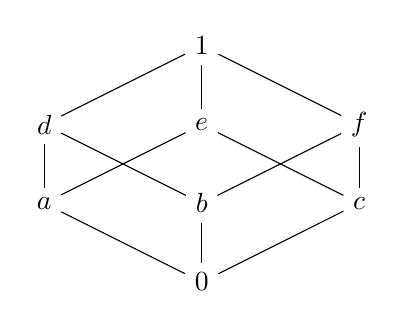
\begin{tikzpicture}[node distance=2cm]
    \node (top) at (0,0) {$1$};

    \node (a) at (-2,-2) {$a$};
    \node (b) at (0, -2) {$b$};
    \node (c) at (2, -2) {$c$};

    \node (d) at (-2, -1) {$d$};
    \node (e) at (0, -1) {$e$};
    \node (f) at (2, -1) {$f$};

    \node (bottom) at (0,-3) {$0$};

    \draw (bottom) -- (a);
    \draw (bottom) -- (b);
    \draw (bottom) -- (c);

    \draw (a) -- (e);
    \draw (c) -- (e);

    \draw (a) -- (d);
    \draw (b) -- (d);

    \draw (b) -- (f);
    \draw (c) -- (f);

    \draw (d) -- (top);
    \draw (e) -- (top);
    \draw (f) -- (top);

  \end{tikzpicture}
\end{center}

\tableofcontents
\newpage
\section{Introduction}
\label{sec:Introduction}
\subsection{Lattices}
\label{subsec:Introduction-Lattices}
A lattice $\calC$ is a poset \st for any pair $(a,b) \in \calC$, the supremum $a \land b$, and infimum $a \lor b$ exist. We extend this to a complete lattice, which has the requirement that for any subset $\calD \subseteq \calC$ the supremum $\bigvee \calD$ and infimum $\bigwedge \calD$ exist. 

\subsection{Formal Contexts}
\label{subsec:Introduction-Formal_Contexts}
A Formal Context is a triple $\langle G, M, I \rangle$ where $G$ refers to a set of objects, $M$ to a set of properties, and $I$ an incidence relation over $G\times M$. 

We have derivation operators $A'$ and $B'$; for $A'$, where $A \subseteq G$, the derivation operator tells us which properties belong to the objects in $A$, the dual holds for properties and their objects. \textbf{Formally}, 

\begin{definition}
    \[ A' := \left\{m \in M \,|\, \forall g \in A, gIm\right\} \]
    \[ B' := \left\{g \in G \,|\, \forall m \in B, gIm\right\} \]
\end{definition}

We also have closure operators, $A''$, which works intuitively by applying the derivation operator on $A$ ($B$), which yields a set of properties. Then applying it again on $A'$ ($B'$), which yields back a set of objects (properties). 

\begin{proposition}
    For subsets $A, B\subseteq G$ (defined dually for properties $C,D \subseteq M$), we have
    \begin{itemize}
        \item[a.] $A \subseteq B \implies B' \subseteq A'$ 
        \item[b.] $A \subseteq A''$ 
        \item[c.] $A' = A'''$
    \end{itemize}
\end{proposition}

For more natural discussion, \textit{a} describes the behaviour that if we have two sets of objects $A$ and $B$, where $A \subseteq B$; then it follows that objects in $A$ will have at \textit{least} all the properties of objects in $B$. 

\subsection{Formal Concepts}
\label{sec:Introduction-Formal_Concepts}

\textit{Presume we are working with a formal context $\langle G, M, I \rangle$.}
\begin{definition}
    
    $(A,B)$ is a \textit{\textbf{formal concept}} of our formal context \textit{iff}    $A \subseteq G$, $B \subseteq M$, $A' = B$, and $B' = A$ 
\end{definition}

$A$ is called the \textbf{extent}, and $B$ is called the \textbf{intent}. We can refer to the set of all formal concepts of a formal context as a $\calB (G, M, I)$.
\section{Closure Systems}
\label{sec:Closure_Systems}

\subsection{Defining a Closure System}
\label{subsec:Closure_Systems-Defining_a_Closure_System}

If we are given a set $M$, a closure system $\calC$ on $M$ is a set of subsets of $M$ ($\calC \subseteq \mathcal{P}(M)$) for which: 

\begin{itemize}
    \item $M \in \calC$
    \item if $D\subseteq \calC$ then, $\bigcap D \in \calC$
\end{itemize}

We might observe that the first point is ensured by the second point; this is because $\bigcap \emptyset = M$ - if we don't have this property, we have a contradiction. We might also observe that a closure system has a natural ordering; specifically, by subsumption. That is, $\calC$ is a poset with $(\calC, \subseteq)$. 

\subsection{Closure Operators}
\label{subsec:Closure_Systems-Closure_Operators}

\section{Implications}
\label{sec:Implications}

\subsection{Introduction}
If $M$ is a set of attributes, we say that $A \rightarrow B$ is an implication over $M$; $A,B \subseteq M$. A set $D\subseteq M$ respects an implication $A \rightarrow B$ if i) $A \not \subseteq D$ or ii) $B \subseteq D$ - the same as material implication. We can represent this notion as $D \models A \rightarrow B$. 

If we have a set of implications $L := \{I_1,\dots ,I_n\}$ we say that a subset $D \models L$ if it respects every implication in $L$: formally, $D \models L \iff \forall A \rightarrow B \in L, D \models A \rightarrow B$. 

\subsubsection{Implications in a Formal Context}
Suppose we have a formal context $\mathcal{K} := (G, M, I)$ and $A \rightarrow B$ where  $A, B \subseteq M$. We say that $K \models A \rightarrow B$ if $\forall g \in G, g' \models A \rightarrow B$. That is, a formal context is a model of some implication, if every object in $G$ has a intent which is a model of that implication. 

Given $K \models A \rightarrow B$, the following are equivalent: 
\[1. \forall g \in G, g' \models A\rightarrow B \]
\[2. B \subseteq A''\]
\[3. A' \subseteq B'\]

(1) is obvious. 

For (2), we need to show $K \models A \rightarrow B \iff B \subseteq A''$. 

$\Rightarrow$ We want to show that $\forall g \in G, g' \models A \rightarrow B \implies B \subseteq A''$ 
\begin{enumerate}
    \item Every object which has $A$ in its intent, also has $B$ in its intent. 
    \item This means, $\forall g \in G, A \subseteq g', B \subseteq g'$
    \item So $B$ is a subset of every object intent in $G$. 
    \item Thus, $B \subseteq A''$. 
\end{enumerate}

$\Leftarrow$ Show that $B \subseteq A'' \implies \forall g \in G, g' \models A \rightarrow B$. 
\begin{enumerate}
    \item $A'''$ is the set of objects which have $A$ in their intents
    \item We know that all of these objects will have $B$ in their intents too (assumption)
    \item So, $\forall g \in G$ if $g\in A'''$ then $B \in g'$ and so $g' \models A \rightarrow B$. 
    \item $\forall g \in G$ and $g \not \in A'''$, then $g' \models A \rightarrow B$ trivially. 
    \item $\forall g \in G, g' \models A \rightarrow B$
\end{enumerate}

[We still need to do proof for (3)] 
\clearpage

\subsection{Sets of Implications}
Let $L$ be a set of implications over $M$, then 
\[Mod(L) := \{T \in \mathcal{P}(M) | T \models L\}\]
$Mod(L)$ is the set of all subsets of $M$ which are models of the set of implications $L$. This is a closure system on $M$. We can see that $M \in Mod(L)$ because for any implication $A \rightarrow B$ over $M$, $M \models A\rightarrow B$. 
\begin{proof}
    $M \models A\rightarrow B$ for any implication over $M$ with $A, B \subseteq M$. 
    \begin{enumerate}
        \item Let $A\rightarrow B$ be some implication over $M$. 
        \item Suppose $M \not \models A \rightarrow B$. 
        \item Then $A \subseteq M$ and $B \not \subseteq M$ 
        \item Contradiction, since $A, B \subseteq M$
    \end{enumerate}
\end{proof}
\begin{proof}
    The intersection of any elements in $Mod(L)$ is also in $Mod(L)$. 
    \begin{enumerate}
        \item Let $X, Y \in Mod(L)$, 
        \item Assume $X \cap Y \not \in Mod(L)$, 
        \item Then, for some $A\rightarrow B \in L, X \cap Y \not \models A \rightarrow B$, 
        \item $X \cap Y \subseteq A$ and $X \cap Y \not \subseteq B$. 
        \item But $Mod(L)$ is such that $\forall m \in Mod(L), A \subseteq m \implies B \subseteq m$. 
        \item If $X \cap Y \subseteq A$ then $X \cap Y \subseteq B$. 
        \item Thus, $X \cap Y \in Mod(L)$
    \end{enumerate}
\end{proof}

The above proves that $Mod(L)$ is a closure system on $M$. (From the definition in \ref{sec:Closure_Systems}) If L is the set of all implications of a formal context, then $Mod(L)$ is the system of all concept intents. 

Since $Mod(L)$ is a closure system, we have a closure operator $X \mapsto L(X)$, which can be described in two ways. 

$X^\mathcal{L} := X \cup \bigcup\{B | A \rightarrow B \in \mathcal{L}, A \subseteq X\}$. 

We then keep applying $X^\mathcal{L}$ until we get a fixed point $\mathcal{L}(X) := X^{\mathcal{L}\dots \mathcal{L}}$ with $\mathcal{L}(X)^\mathcal{L} = \mathcal{L}(X)$. 

Alternatively, we define the closure operator as $\mathcal{L}(X) := \bigcap\{Y | X \subseteq Y \subseteq M, Y \in Mod(L)\}$ 

These two definitions are equivalent; the first one is an iterative definition, which says: given a subset of $M$, $X$ - keep applying all the implications from $\mathcal{L}$ until we reach a fixed point. The second definition says that we define the closure of $X$ as the intersection between all the models of $\mathcal{L}$ which contain $X$. 
\clearpage

\subsection{When does an implication follow from other ones?}
Let $\mathcal{L}$ be a set of implications, and $A\rightarrow B$ an implication over $M$. How do we know if $\mathcal{L} \models A\rightarrow B$. Or, how do we know if an implication follows semantically from a set of implications? If every subset of $\mathcal{L}$ which respects $\mathcal{L}$ also respects $A\rightarrow B$. 

\begin{proof}
    $\mathcal{L} \models A\rightarrow B \iff B \subseteq \mathcal{L}(A)$

    $\mathcal{L} \models A\rightarrow B \Rightarrow B \subseteq \mathcal{L}(A)$
    \begin{enumerate}
        \item Assume $B \not \subseteq \mathcal{L}(A)$
        \item Then, $\exists Y \in Mod(\mathcal{L})$ \st $A \subset Y$ and $B \not \subseteq Y$.
        \item $Y \not \models A \rightarrow B$ and $Y \in Mod(\mathcal{L})$
        \item Contradiction, since $\mathcal{L} \models A\rightarrow B$
    \end{enumerate}

    $B \subseteq \mathcal{L}(A) \Rightarrow \mathcal{L} \models A\rightarrow B$ by contrapositive.
    \begin{enumerate}
        \item Assume $\mathcal{L} \not \models A \rightarrow B$ 
        \item Then, there exists some element $I \in Mod(\mathcal{L})$ with $A\subseteq I$ and $B \not \subseteq I$. 
        \item By inspection, $I \in \{Y | A \subseteq Y \subseteq M, Y \in Mod(\mathcal{L})\}$
        \item Which would then mean that $B \not \subseteq \bigcap \{Y | A \subseteq Y \subseteq M, Y \in Mod(\mathcal{L})\}$ 
    \end{enumerate}
\end{proof}
\end{document}
